\documentclass[a4paper,12pt]{scrartcl}
\usepackage[ngerman]{babel}
\usepackage[utf8]{inputenc}
\usepackage[T1]{fontenc}
\usepackage{lmodern}
\usepackage{amssymb}
\usepackage{graphicx}
\usepackage{amsmath}
\usepackage{multicol}
\usepackage{enumerate}
\usepackage{verbatim}
\usepackage{pgfplots}
\usepackage{scrpage2}\pagestyle{scrheadings}
\usepackage{tikz}
\usetikzlibrary{patterns}

\newcommand{\titleinfo}{Leistungsanalyse}

\title{\titleinfo}
\author{Sönke Kracht, Sven-Hendrik Haase}
\date{\today}
\chead{\titleinfo}
\ohead{\today}
\setheadsepline{1pt}
\setcounter{secnumdepth}{0}
\newcommand{\qed}{\quad \square}

\begin{document}
\maketitle
\notag

\subsection{Communication A}
\subsubsection{Gauss-Seidel}
\begin{multicols}{2}
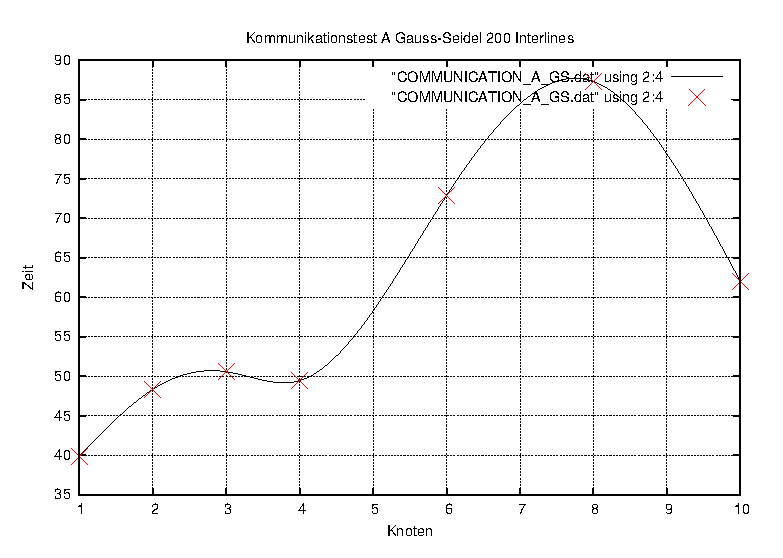
\includegraphics[scale=0.5]{results/COMMUNICATION_A_GS.eps}
\verbatiminput{results/COMMUNICATION_A_GS.dat}
\end{multicols}

In diesem Graphen sieht man eine Korrelation zwischen benötigter Zeit
und Anzahl der Knoten mit 12 Prozessen, auf dem das Programm
gleichzeitig ausgeführt wurde. Die benötigte Zeit nimmt tendenziell zu.
Bei 3 Knoten lässt sich ein lokales Maximum beobachten, bei 4 Knoten
ein lokales Minimum und bei 8 Knoten ein globales Maximum.
Bei 10 Knoten nimmt die benötigte Zeit wieder rapide ab.
Der Anstieg der Zeit im Allgemeinen
lässt sich dadurch erklären, dass bei mehr Nodes der
Aufwand der Kommunkation wächst.

\newpage

\subsubsection{Jacobi}
\begin{multicols}{2}
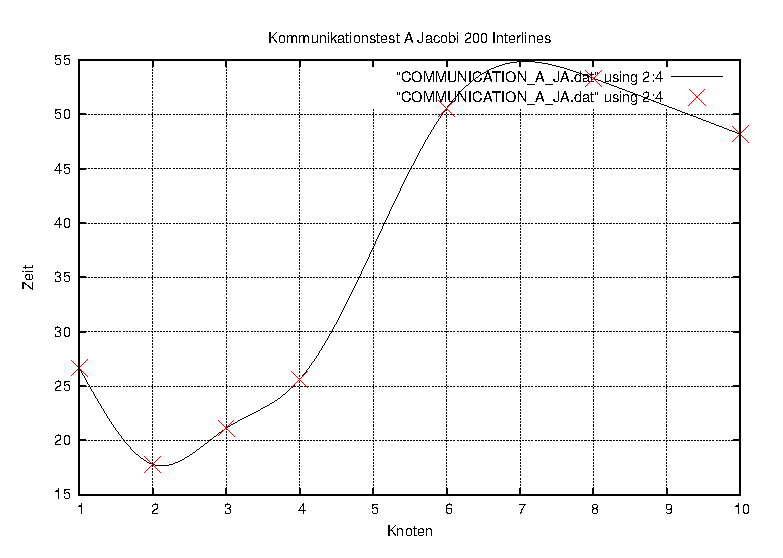
\includegraphics[scale=0.5]{results/COMMUNICATION_A_JA.eps}
\verbatiminput{results/COMMUNICATION_A_JA.dat}
\end{multicols}

Dieser Graph zeigt die gleichen Daten wie der vorherige und verhält sich
ähnlich.

\subsection{Communication B}
\subsubsection{Gauss-Seidel}
\begin{multicols}{2}
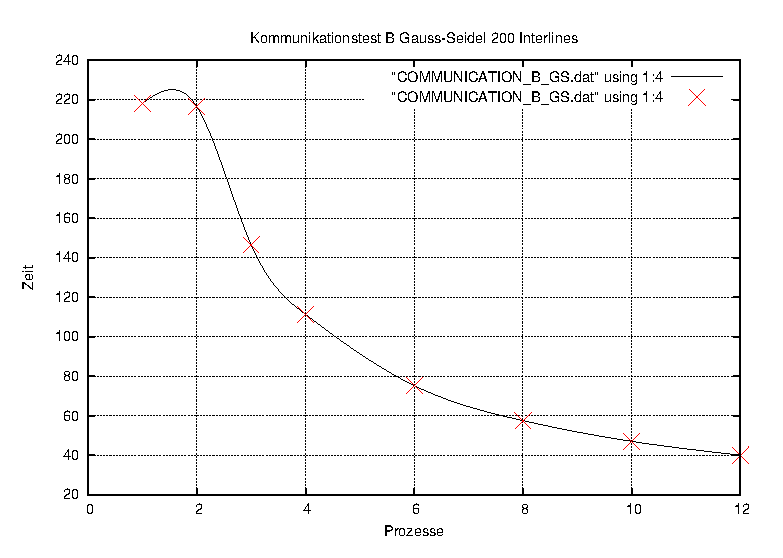
\includegraphics[scale=0.5]{results/COMMUNICATION_B_GS.eps}
\verbatiminput{results/COMMUNICATION_B_GS.dat}
\end{multicols}

In diesem Graphen sieht man eine Korrelation zwischen benötigter Zeit
und Anzahl der Prozesse aus einem einzigen Knoten. Die benötigte Zeit
nimmt mit wachsender Prozesszahl stetig ab. Bei einem Prozess und zwei
Prozessen besteht ca. die gleiche Laufdauer, da bei einem Prozess die
gesamte Kommunikation entfällt, die erst ab zwei Prozessen hinzukommt.
Die abschließende Synchronisation der Pipeline nimmt ebenfalls Zeit in
Anspruch.

\newpage

\subsubsection{Jacobi}
\begin{multicols}{2}
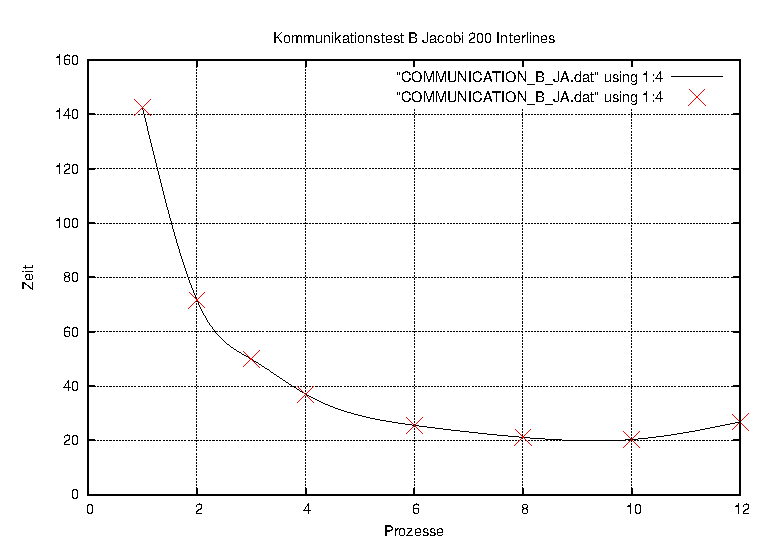
\includegraphics[scale=0.5]{results/COMMUNICATION_B_JA.eps}
\verbatiminput{results/COMMUNICATION_B_JA.dat}
\end{multicols}

Dieser Graph zeigt die gleichen Daten wie der vorherige und verhält sich
ähnlich. Bei zwei Prozessen ist im Vergleich zu Gauss-Seidel ein Speedup
zu beobachten, da der Kommunikationsaufwand nicht so schwer ins Gewicht fällt.

\newpage

\subsection{Communication C}
\subsubsection{Gauss-Seidel}
\begin{multicols}{2}
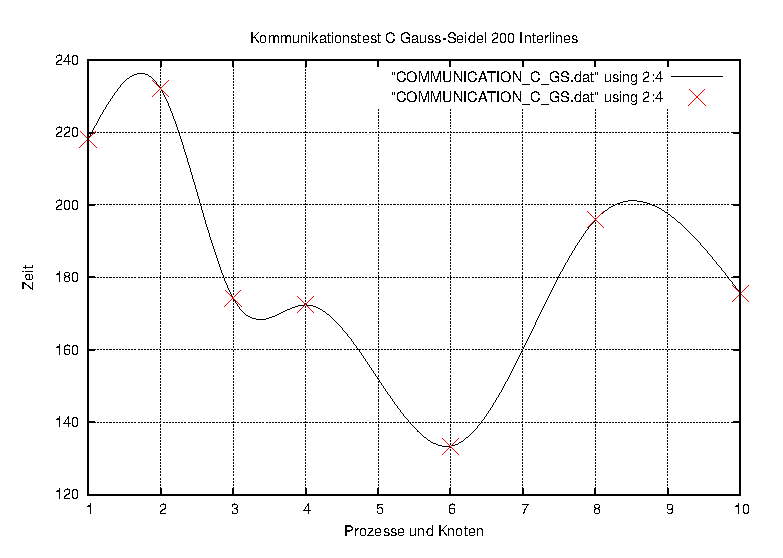
\includegraphics[scale=0.5]{results/COMMUNICATION_C_GS.eps}
\verbatiminput{results/COMMUNICATION_C_GS.dat}
\end{multicols}

Dieser Graph zeigt die Korrelation zwischen benötigter Zeit und
der Anzahl der Prozesse bzw. Knoten (Prozesszahl == Knotenzahl).
Allgemein ist zu beobachten, dass eine Talform vorliegt. Ein globales
Maximum liegt bei zwei Prozessen bzw. Knoten, ein globales Minimum bei 6
und dann wieder ein lokales Maximum bei 8.

\subsubsection{Jacobi}
\begin{multicols}{2}
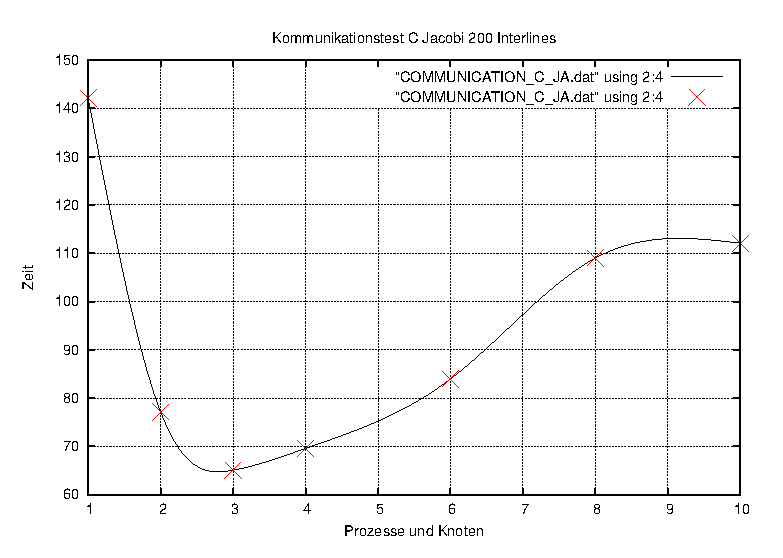
\includegraphics[scale=0.5]{results/COMMUNICATION_C_JA.eps}
\verbatiminput{results/COMMUNICATION_C_JA.dat}
\end{multicols}

Dieser Graph präsentiert die gleichen Daten wie der vorherige Graph.
Er weist ein grob ähnliches Verhalten auf. Auch hier wieder sieht man das Tal.
Das globale Maximum liegt bei 1. Das globale Minimum liegt bei 3 und das
lokale Maximum bei 10.

\newpage

\subsection{Weak Scaling}
\subsubsection{Gauss-Seidel}
\begin{multicols}{2}
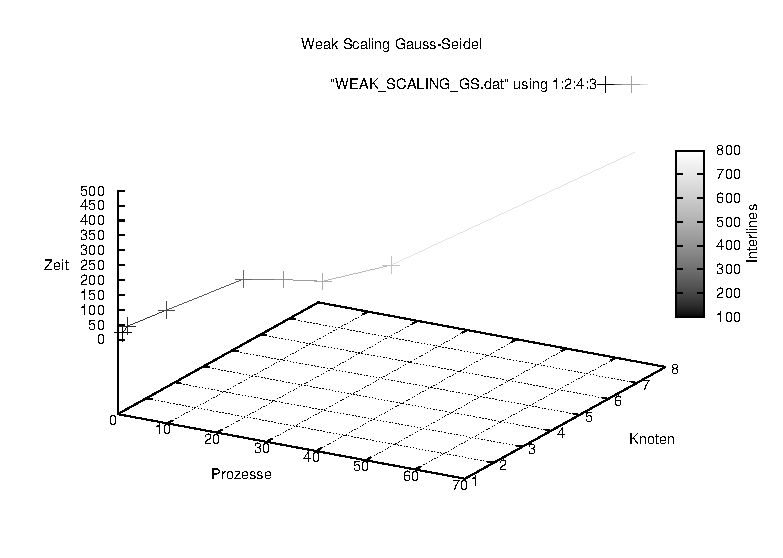
\includegraphics[scale=0.5]{results/WEAK_SCALING_GS.eps}
\verbatiminput{results/WEAK_SCALING_GS.dat}
\end{multicols}


Diesr Graph korreliert die Anzahl der Prozesse, Knoten, Interlines und der 
Zeit. Diese Tatsache macht eine Interpretation schwierig. Allgemein lässt 
sich aber beobachten, dass der Speedup bescheiden ausfällt.

\subsubsection{Jacobi}
\begin{multicols}{2}
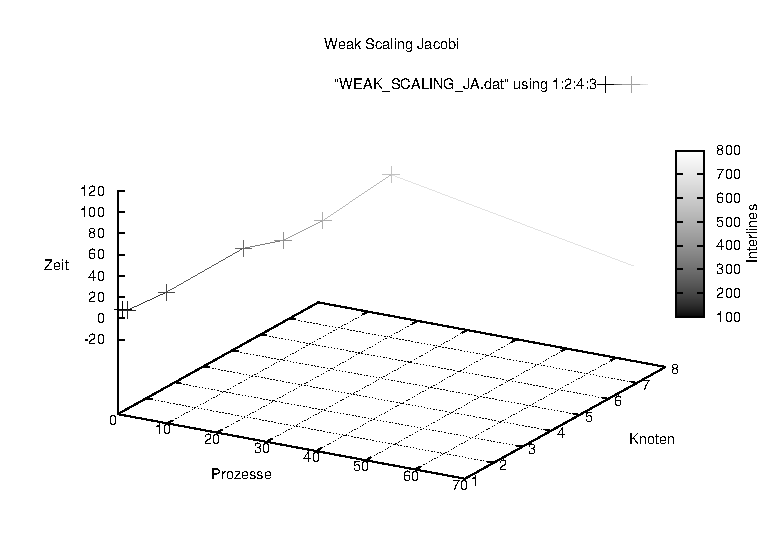
\includegraphics[scale=0.5]{results/WEAK_SCALING_JA.eps}
\verbatiminput{results/WEAK_SCALING_JA.dat}
\end{multicols}

Hier lassen sich alle wesentlichen Eigenschaften des oberen Graphen noch 
einmal beobachten. Dem hinzuzufügen wäre, dass der letzte Wert aufgrund eines 
Timeouts nicht mehr gerechnet wurde.

\newpage

\subsection{Strong Scaling}
\subsubsection{Gauss-Seidel}
\begin{multicols}{2}
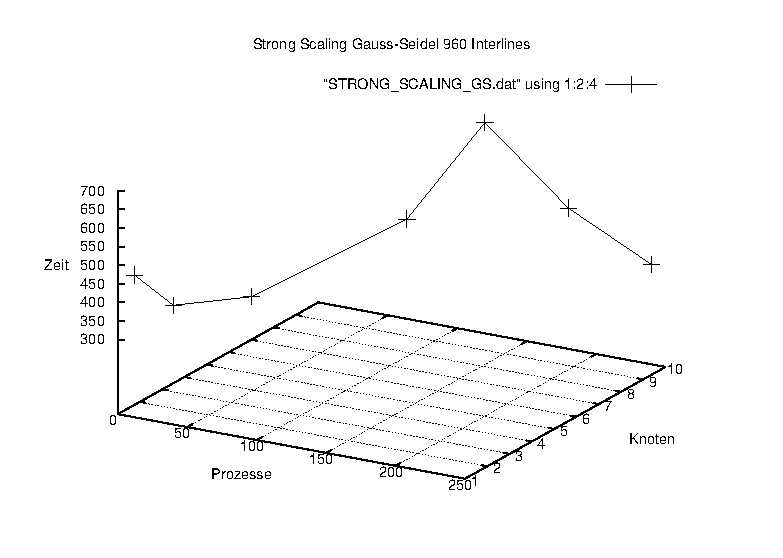
\includegraphics[scale=0.5]{results/STRONG_SCALING_GS.eps}
\verbatiminput{results/STRONG_SCALING_GS.dat}
\end{multicols}

Diser Graph korreliert Prozesse, Knoten und benötigte Zeit. Es lässt sich
beobachten, dass der Speedup im Allgemeinen zwar vorhanden ist, aber selbst
mit einer hohen Anzahl an Prozessen schlecht ausfällt.
Interessant zu bemerken ist, dass ab sich die benötigte Zeit ab 120 Prozessen
mit gleichbleibender Knotenanzahl bis hin zu 240 Prozessen fast halbiert.
Auch hier ist eine Interpretation wieder schwierig.

\subsubsection{Jacobi}
\begin{multicols}{2}
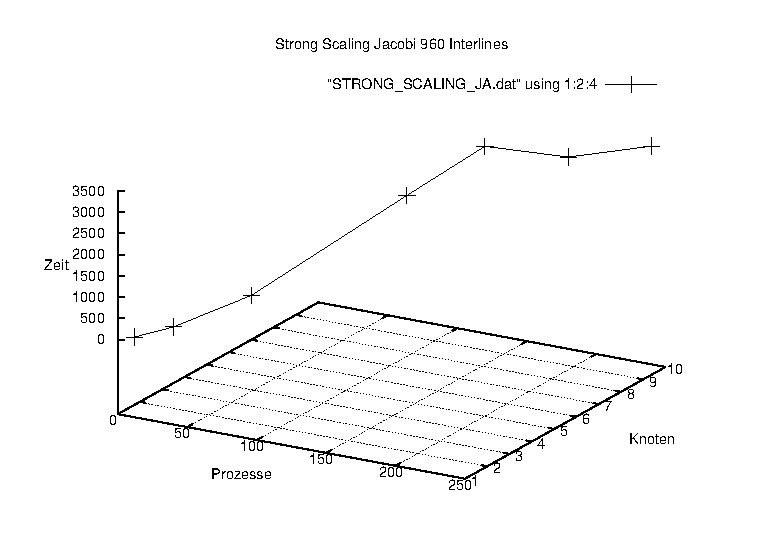
\includegraphics[scale=0.5]{results/STRONG_SCALING_JA.eps}
\verbatiminput{results/STRONG_SCALING_JA.dat}
\end{multicols}

Dieser Graph stellt die gleichen Daten dar wie der vorherige. Es ist zu
beobachten, dass Gauss-Seidel im Vergleich algorithmisch
wesentlich schneller ist als Jacobi.
Ebenfalls profitiert Jacobi offenbar nicht von einer erhöhten Anzahl an
Prozessen.

\end{document}